\subsection{Chromium dimer}

The chromium dimer has been a challenging molecule for quantum chemistry for many years. This
is because a relatively large active (12e, 12o) space  is needed to 
describe the minimal spin-recoupling
of the electrons involved in the nominal sextuple bond, while, at the same time, a large amount of dynamic correlation is  required 
even to yield a bound potential energy curve. \cite{andersson_cr2_1994,roos_multiconfigurational_1995,roos_multiconfigurational_1996,roos_ground_2003,angeli_third-order_2006,muller_large-scale_2009,kurashige_second-order_2011,sharma_multireference_2015}
%Perturbation theory is relatively cheap among methods for dynamic correlation, such as multi-reference couple cluster, multi-reference configuration interaction. It is widely used in the chromium dimmer calculations. 

The minimal (12e,12o) CAS, derived from the 3d and 4s atomic orbitals, has been  widely employed in earlier chromium dimer calculations.\cite{andersson_cr2_1994,roos_multiconfigurational_1995,roos_multiconfigurational_1996,angeli_third-order_2006,muller_large-scale_2009,sharma_multireference_2015} Although these earlier calculations
could reproduce the general shape of the potential energy curve, they
also have a number of shortcomings.
For example,  both CASPT2\cite{andersson_cr2_1994,roos_multiconfigurational_1995,roos_multiconfigurational_1996} and NEVPT2\cite{angeli_n-electron_2001} based on the CASSCF(12e,12o) reference function  significantly overestimate the 
dissociation energy of the molecule, especially when large basis sets (e.g. those including g-, h-, or i- type functions) are used.\cite{celani_cipt2_2004,angeli_third-order_2006} Further, with NEVPT3, \cite{angeli_third-order_2006} starting
from the CAS(12e,12o) wavefunction  results in a large correction to the NEVPT2 result 
and an unphysical potential energy curve. These various results suggest 
that (at least when used with low orders of perturbation
theory and internally contracted formulations which have a limited ability to relax the reference) the minimal (12e,12o) CAS is too small for a quantitative description.

Further, when using CASPT2, the results are also  sensitive to the choice of the zeroth-order Hamiltonian and
the level shift employed.\cite{celani_cipt2_2004,ruiperez_complete_2011} This is 
especially true for the (12e,12o) active space,
but sensitivity can still be seen even in  DMRG-CASPT2 calculations with a large (12e,28o) CAS derived from the 3$d$, 4$s$, 4$p$, 4$d$ atomic orbitals.~\cite{kurashige_second-order_2011}
While the large active space DMRG-CASPT2 curves are generally close to the experimentally derived
 curve, the different choices of zeroth-order level shifts 
still yielded a variation in $D_e$ 
of about 0.2~eV.~\cite{kurashige_second-order_2011} Since NEVPT2 does not require level shifts to avoid intruders, the above provides further incentive
to recompute the chromium dimer potential energy curve using DMRG-SC-NEVPT2,
and with a large active space.

\begin{figure}
  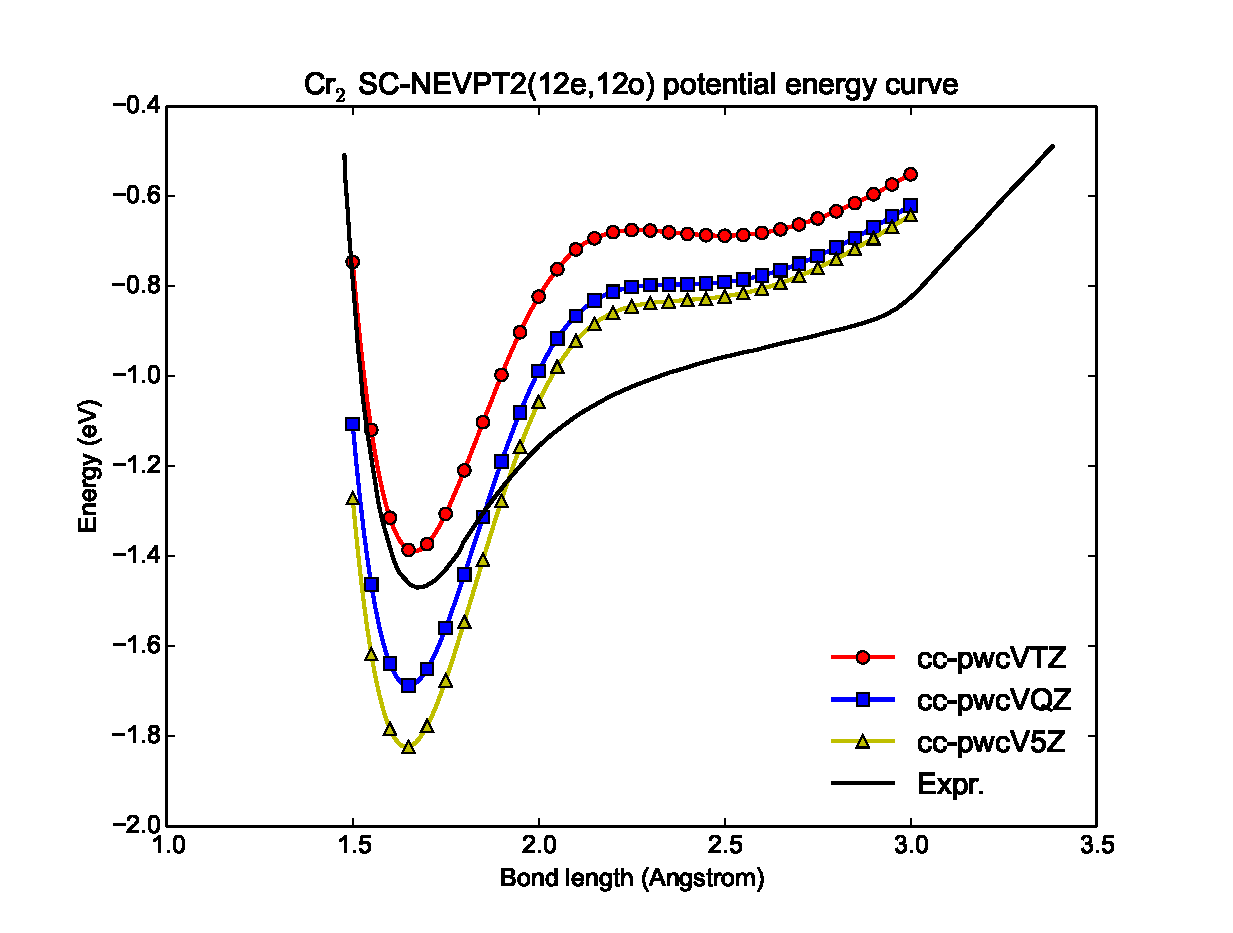
\includegraphics[width=1.1\columnwidth]{Cr2-nevpt2.eps}
  \caption{SC-NEVPT2(12e,12o) potential energy curve with a suite of cc-pwCVXZ (X=T,Q,5) basis sets. \textcolor{red}{Change ``Expr.'' to ``Expt.'',
  cc-pwcvXZ -- cc-pwCVXZ.}}
  \label{fig:12o_nevpt2}
\end{figure}

For our DMRG-SC-NEVPT2 calculations, we used a suite of cc-pwcVXZ (X = T,Q,5) basis sets. No basis set superposition error (BSSE) corrections were applied 
due to the large basis sets used (which included h- and i-type functions). The X2C Hamiltonian was used to describe scalar relativistic effects. 
The DMRG reference and corresponding RDM and DMRG-SC-NEVPT2 calculations were performed using the \textsc{Block} program\cite{sharma_spin-adapted_2012}. 
All other calculations were performed in \textsc{Pyscf} \cite{sun_pyscf}. In the figures, the energy of the isolated atoms is set to zero.
%The symmetry of an isolated atom was set as $C_{\infty v}$, while the dimer's symmetry is set as $D_{\infty h}$. Otherwise, the isolated atom's CAS(6e,9o) will be not consistent with the CAS for the dimer.

We first show the SC-NEVPT2(12e,12o) potential energy curve of Cr$_2$ in Figure \ref{fig:12o_nevpt2} 
to demonstrate the basis set convergence with the cc-pwCVXZ bases. The (12e,12o) active space was obtained from a CASSCF calculation. We find that
using larger basis sets together with this small active space indeed yields far too deep a curve, in agreement with earlier studies  using atomic natural orbital (ANO) basis sets.\cite{angeli_third-order_2006}

We then extended the (12e,12o) active space by adding another set of $\sigma$, $\pi$, $\pi'$, $\delta$, $\delta'$ orbitals and their corresponding anti-bonding orbitals 
to obtain a (12e,22o) active space. We selected the orbitals from the converged (12e,12o) CASSCF calculation based on symmetry and their orbital energies,
and the orbitals were then further optimized using DMRG-CASSCF ($M$=1000, no frozen core). Although the additional active orbitals contained both $4p$ and $4d$ character at first, 
the fully optimized additional active orbitals were mainly of $4d$ character.  This is not surprising, as a $4d$ double shell is well known to greatly improve transition metal CAS results~\cite{andersson_excitation_1992}.
From the DMRG-CASSCF optimized orbitals, we then carried out a final larger DMRG calculation with $M$=4000 to obtain an accurate reference wavefunction.
The resulting DMRG reference energy in the active space is accurate to better than 0.1 m$E_h$.
To compute the RDM's for the DMRG-SC-NEVPT2 calculation, the large bond dimension reference MPS was compressed down to an MPS with $M'$=800. 
Finally, the (TZ/QZ/5Z) energies were extrapolated to the complete basis set (CBS) limit using
an exponential formula for the DMRG-CASSCF energy, and an $l^{-3}$ formula for the DMRG-SC-NEVPT2 correction, where $l$ is the maximum angular momentum
of the basis.

\begin{figure}
  \centering
  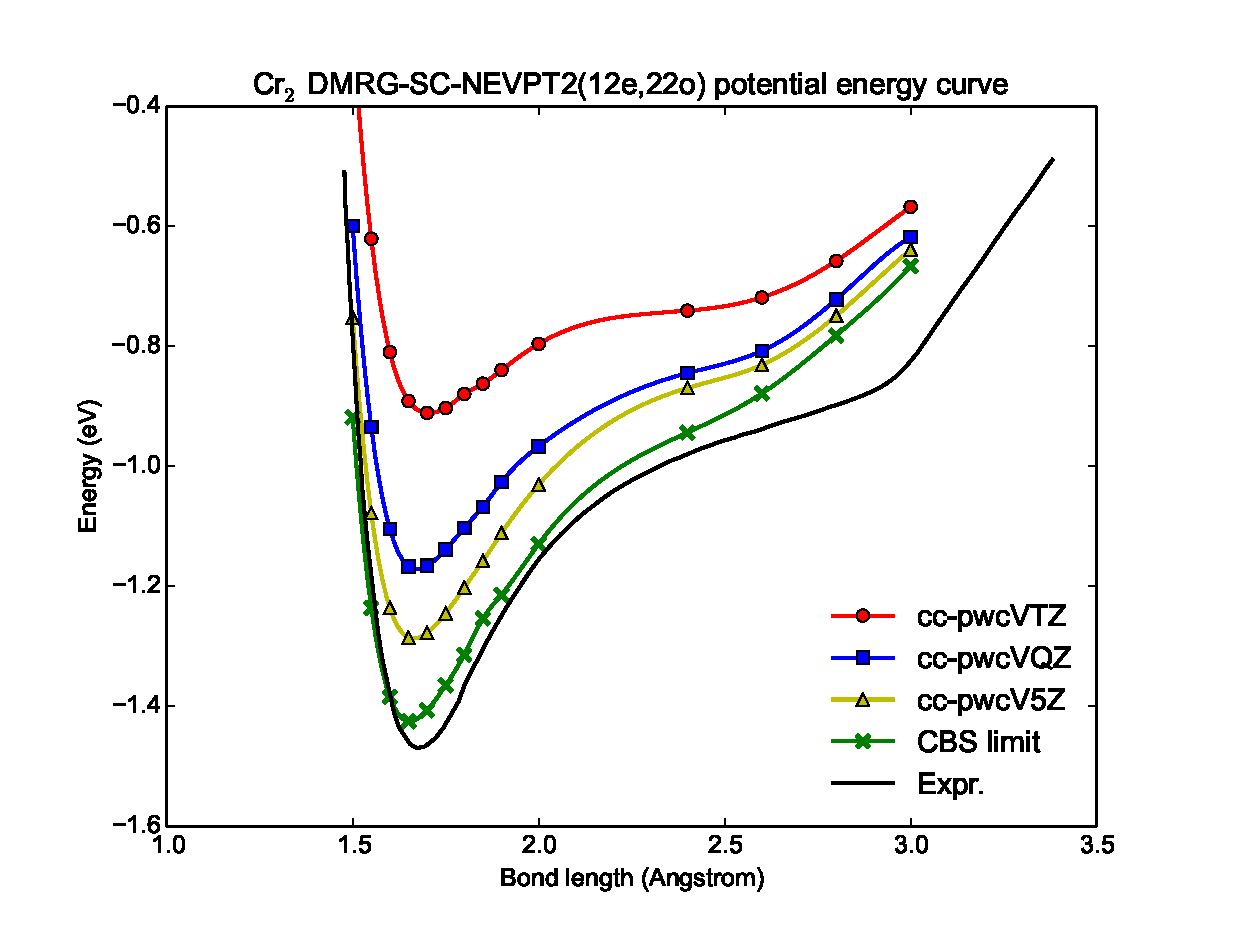
\includegraphics[width=1.1\columnwidth]{Cr2-dmrg-nevpt2.eps}
  \caption{Extended active space DMRG-SC-NEVPT2(12e,22o)($M'$=800) potential energy curves with a suite of cc-pwCVXZ (X=T,Q,5) basis sets,
    and the extrapolated CBS limit. The extended active space includes a double $d$ shell. \textcolor{red}{Capitalize C i.e. cc-pwCVXZ; Expr.-- Expt.}
The experimental curve is taken from Ref.~\onlinecite{casey_negative_1993}.}
  \label{fig:dmrg-nevpt2}
\end{figure}
\begin{figure*}
  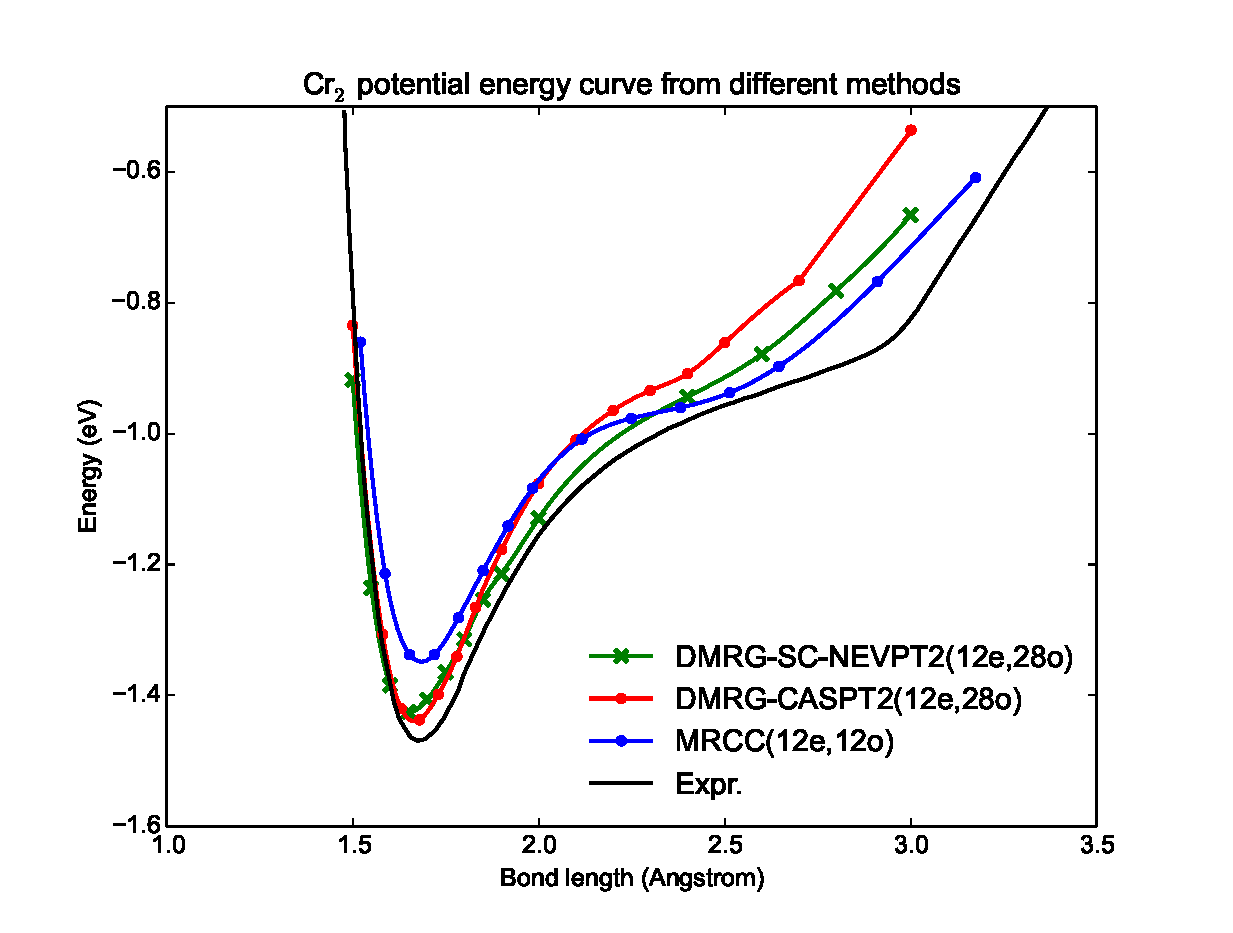
\includegraphics[width=1.5\columnwidth]{Cr2-curves.eps}
  \caption{Cr$_2$ potential energy curves from different methods.  The DMRG-CASPT2(12e,28o) curve is from Ref.~\onlinecite{kurashige_second-order_2011} and the MR-AQCC(12e,12o) curve is from Ref.~\onlinecite{muller_large-scale_2009}. \textcolor{red}{NEVPT2 act. space is wrong, Expr.-- Expt.}}
  \label{fig:compare}
\end{figure*}

Figure \ref{fig:dmrg-nevpt2} shows the potential energy curves obtained with the cc-pwCVXZ (X=T,Q,5) basis sets and the X2C Hamiltonian, as well as the extrapolated
CBS curve. A comparison of the CBS curve to curves obtained with other
correlation methods is shown in Fig.~\ref{fig:compare}.
We see that larger basis sets using this active space yield systematically improved curves, and that
the CBS potential energy curve now agrees very well with the experimental curve, over a wide range of distances. The only significant deviation occurs near the bend at about 2.8\AA, where the reliability of the RKR potential  has previously been questioned.\cite{roos_ground_2003}
The spectroscopic constants are shown in Table \ref{tab:spectro}.
Our obtained CBS $D_e$ of 1.43eV is very close to the inferred experimental binding energy of 1.47 eV from
the negative ion photoelectron spectroscopy measurements
of Casey and Leopold \cite{casey_negative_1993}, while the bond-length and vibrational frequency also agree well. It is remarkable to see that even
with the largest cc-pwCV5Z basis, the binding energy is still 0.14 eV away from the CBS limit,  demonstrating the very large basis set 
effects in this system.  

Compared to earlier ``accurate'' calculations, the computed DMRG-SC-NEVPT2 curve 
here compares  quite favourably. For example, near the equilibrium
distance, the DMRG-SC-NEVPT2(12e,22o) curve is almost identical to the DMRG-CASPT2(12e,28o) curve\cite{kurashige_second-order_2011}. However, in the stretched $4s$ bonding (``shoulder'') region, the DMRG-SC-NEVPT2(12e,22o) curve is much closer to the experimental one. This seems consistent with the increased correlation strength in the $4s$ bonding region, which could be harder to describe with the simpler zeroth order Hamiltonian employed in CASPT2. Across the full range of distances, the DMRG-SC-NEVPT2 curve also appears considerably more accurate than the MR-AQCC(12e,12o) curve, likely due to the larger active space employed.

The (12e,28o) CAS used in the earlier DMRG-CASPT2 calculations 
contained $4p$ orbitals. However, the accuracy of the DMRG-SC-NEVPT2(12e,22o) curve as compared to the DMRG-CASPT2(12e,28o), together with the fact that only $4d$ orbitals remain in the active space after orbital optimization, suggests that the $4d$ orbitals are more important than the $4p$ orbitals in the correlations of this system. It has also been suggested in some studies
that semi-core correlations (involving the $3s$ and $3p$ orbitals) should also have  a large effect. In Fig.~\ref{fig:semicore} we show the corresponding curves
computed using a (28e,20o) active space containing the semi-core $3s, 3p$ orbitals and $3d, 4s$ valence shell (but no $4d$ shell). We see that the curves are in fact much worse than the curves obtained with the (12e,22o) active space above. This 
indicates double shell correlations are more important than 
the semi-core correlations in this system, and that the latter are well accounted for at the second-order perturbation theory level.

\begin{figure}
  \centering
  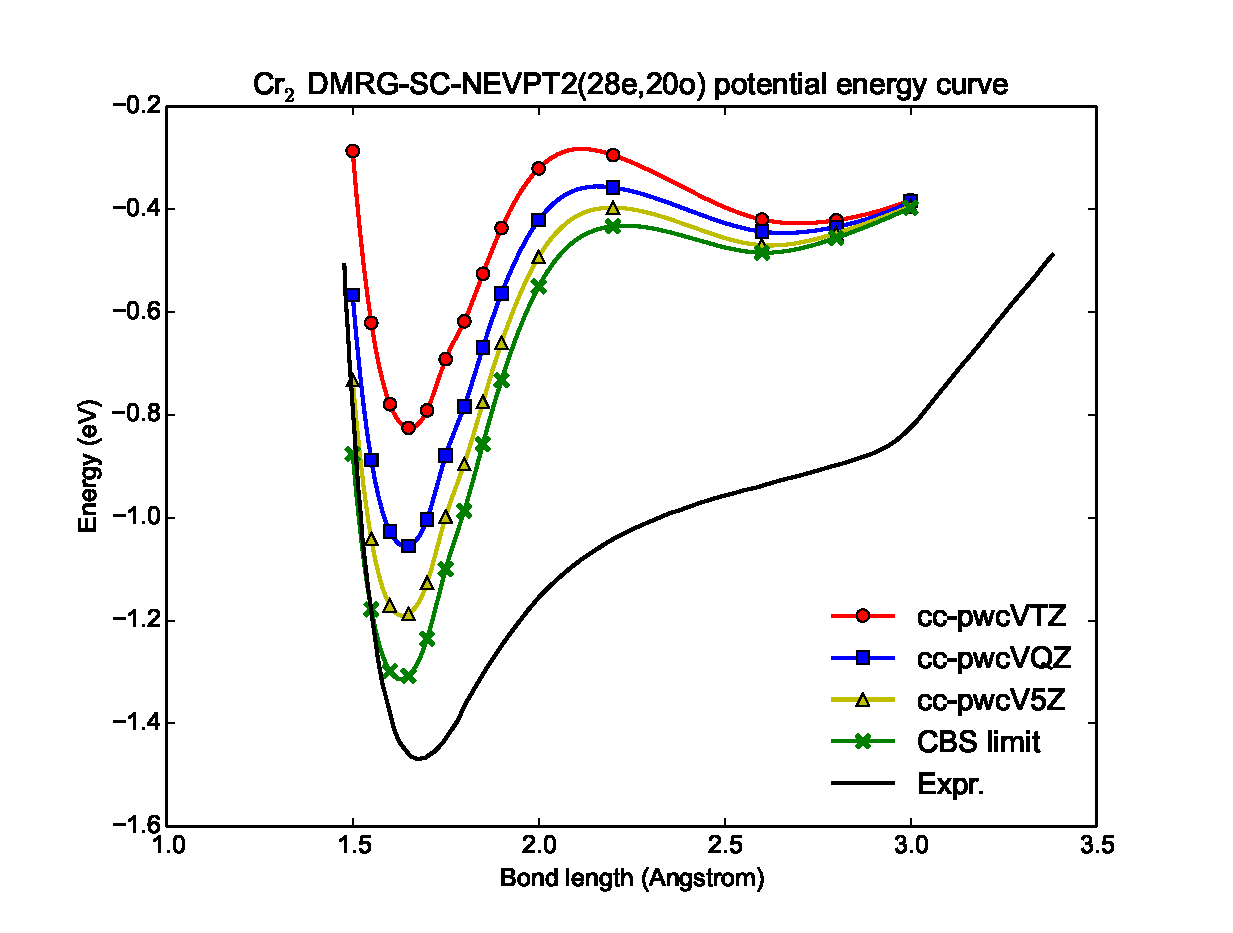
\includegraphics[width=1.1\columnwidth]{Cr2-dmrg-nevpt2_semicore.eps}
  \caption{Extended semi-core DMRG-SC-NEVPT2(28e,20o)($M'$=800) potential energy curve with a suite of cc-pwCVXZ (X=T,Q,5) basis sets, and the extrapolated CBS limit. The semi-core space includes the 3$s$ and 3$p$ shells. 
The experimental curve is taken from Ref.~\onlinecite{casey_negative_1993}.}
  \label{fig:semicore}
\end{figure}

 \begin{table}
\caption{Spectroscopic constants for the ground state of Cr$_2$ using different methods.  \label{tab:spectro}}
  \begin{tabular}{cccc}
  \hline
  & $D_e(eV)$ & $R_0($\AA$)$ & $\omega_e$(cm$^{-1}$ \\
  \hline
  %DMRG-SC-NEVPT2(12e,22o)(M=500) & 1.427 & 1.655 & 486 \\ 
  DMRG-SC-NEVPT2(12e,22o) \footnote{From fitting the energies at five points, R=1.60,1.65, 1.70, 1.75, and 1.80 \AA}&  & & \\
  M=800 & 1.425 & 1.654 & 482 \\ 
  M=1200 & 1.429 & 1.656 & 471 \\ 
  DMRG-CASPT2(12e,28o)\footnote{DMRG-CASPT2(12e,28o)/{\bf $g_1$}($M=\infty$) with the cc-pwCV5Z basis set in Ref.~\onlinecite{kurashige_second-order_2011}} & 1.610 & 1.681 & 480 \\
  MR-AQCC(12e,12o)\footnote{TZP/QZP CBS limit in Ref.~\onlinecite{muller_large-scale_2009}} & 1.355 & 1.685 & 459 \\
  FP-AFQMC\footnote{Ref.~\onlinecite{purwanto_auxiliary-field_2015}} & 1.63(5) & 1.65(2) & 552(93) \\
  experiment & 1.47(5)\footnote{\label{fn:note1}Ref.~\onlinecite{casey_negative_1993}} & 1.679\footnote{Ref.~\onlinecite{bondybey_electronic_1983}} & 480.6(5)\footref{fn:note1} \\
  & 1.47 $\pm$0.1 \footnote{Ref.~\onlinecite{su_bond_1993}}& &\\ 
  \hline
  \end{tabular}
\end{table}

